\chapter{Cookbook}
\label{section:cookbook}

In this chapter the reader will learn about the webaccess architecture by example. 

\section{Folder details plugin}
\label{section:folderdetails}

Our first task is to write a simple plugin that shows the status of the currently selected folder.
As the user selects folders from the hierarchy tree on the left of the screen a line of text
in the bottom toolbar is updated, showing the number of total and unread items in the folder.
The screen shot in Figure \ref{figure:plugin} shows the component in action. The finished
implementation can be found in the source tree in {\tt Zarafa.plugins.FolderStatus}.

\begin{figure}[h!]
\centering
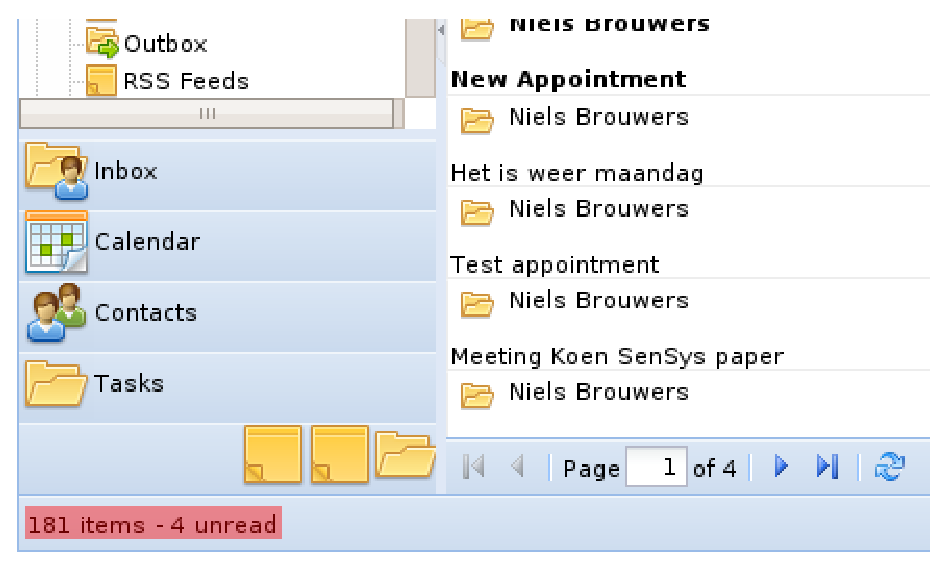
\includegraphics[width=9cm]{figures/plugin.eps}
\caption{Folder status plugin.}
\label{figure:plugin}
\end{figure}

We will start by writing some boilerplate, shown in Listing \ref{listing:plugin1}. The class 
{\tt Zarafa.plugins.FolderStatus} is declared, extending {\tt Zarafa.ui.Plugin}
\footnote{More info on OO and ExtJS can be found at http://www.extjs.com/learn/Manual:Intro}.
Each registered plug-in has a name, so the name 'folderstatus' is passed to the parent
constructor. On line 11 a single instance of this plugin is created and registered with the
global container. For convenience we add an {\tt init} method that is called right
after the parent constructor.

\begin{lstlisting}[caption={Plugin boilerplate}, label=listing:plugin1]
Zarafa.plugins.FolderStatus = function()
{
	config = { name : 'folderstatus' };
	Zarafa.plugins.FolderStatus.superclass.constructor.call(this, config);
	
	// Initialise the plug-in.
	init();
};

Ext.extend(Zarafa.plugins.FolderStatus, Zarafa.ui.Plugin, {

	init : function()
	{
		this.registerInsertionPoint('statusbar.left', this.createFolderStatus, this);
	},
	
	createFolderStatus : function(insertionPoint)
	{
		// Create a new toolbar text item.
		this.textItem = new Ext.Toolbar.TextItem({});
		this.textItem.setText('Hello World!');

		return this.textItem;
	}

});

container.registerPlugin(new Zarafa.plugins.FolderStatus());
\end{lstlisting}

In order to get something on screen we need to hook into an insertion point 
(see Section \ref{section:insertionpoints}). We hook into the {\tt statusbar.left} insertion
point, which is located on the bottom bar, on the left-hand side (see Figure \ref{figure:plugin}).
A component creation function is registered to this insertion point using {\tt registerInsertionPoint}.
Remember that the last line of the listing is executed at 'load' time, so the function 
{\tt createFolderStatus} is registered at that time. It is \emph{called} later, when the UI hierarchy 
is constructed. This function constructs a single UI component, a toolbar text item with the text 
'Hello World!'. 
Running this code results in Figure \ref{figure:plugin2}.

\begin{figure}[h!]
\centering
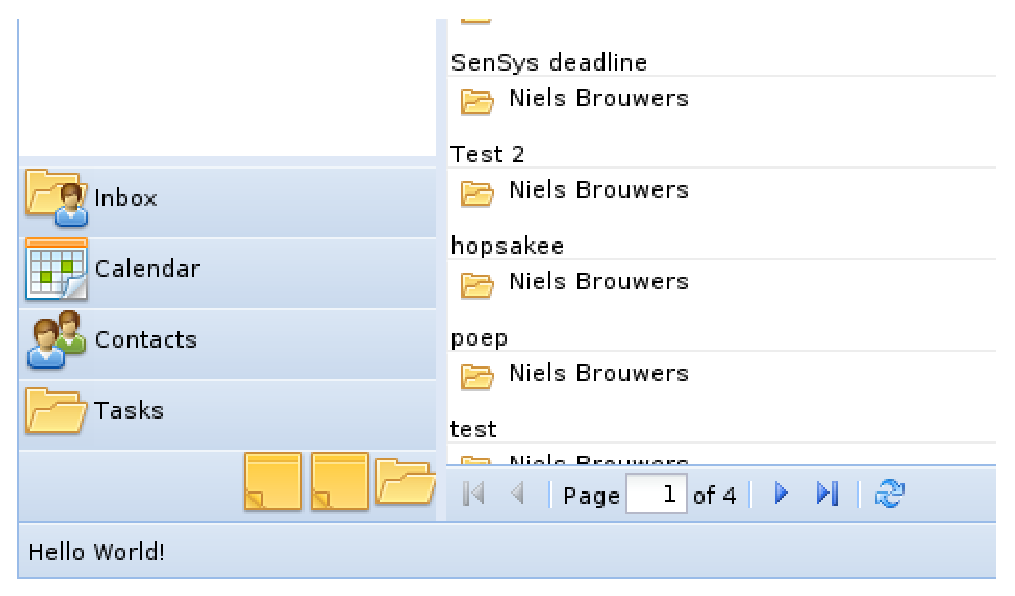
\includegraphics[width=9cm]{figures/plugin2.eps}
\caption{Folder status plugin.}
\label{figure:plugin2}
\end{figure}

Now that we have successfully added a UI component to the interface we would like it to show something
useful. We would like our plugin to display information about the folder that is currently selected.
The {\tt container} object has a {\tt folderselect} event that fires when the user selects a folder.
By listening for this event we can automatically update the text of our text item in the toolbar.

\begin{lstlisting}[caption={Attaching an event handler to the container.}, label=listing:plugin2]
init : function()
{
	this.registerInsertionPoint('statusbar.left', this.createFolderStatus, this);
	
	// Hook into the folder select event of the container
	container.on('folderselect', this.folderSelect, this);
},

updateFolderText : function(store, folder)
{
	// Set the text item text.
	this.textItem.setText(String.format("{0} items - {1} unread",
		folder.content_count,
		folder.content_unread
	));
},

folderSelect : function(store, folder)
{
	// Update the text item with the current store and folder.
	this.updateFolderText(store, folder);
},
\end{lstlisting}

The changed functions are shown in Listing \ref{listing:plugin2}. The event is hooked in {\tt init}, so that
{\tt folderSelect} is called when the user clicks a folder. This method in turn calls {\tt updateFolderText}
which updates the text on the toolbar text item.

The final touch to this plug-in is automatically updating the text when the contents of the folder change due
to user actions such the removal or creation of items. This is left as an exercise to the reader (hint: have
a look at Zarafa.HierarchyModel). The answer can be found in the implementation of 
{\tt Zarafa.plugins.FolderStatus}.

\section{A basic tasks context}
\label{section:taskscontext}

In this example we will build a tasks context. The context will be able to list tasks in a grid control.
We will start by creating a fresh new context called {\tt TaskContext} as shown in Listing 
\ref{listing:taskcontext1}.

Since a context is a type of plug-in the basic structure is similar to the plug-in described in Section
\ref{section:folderdetails}. There are three functions that are defined in the {\tt Context} class 
that every context must override. The {\tt bid} method implements the bidding scheme described in 
Section \ref{section:contexts}. The {\tt createContentPanel} and {\tt createToolbar} methods create 
the neccesairy UI components. 

The bidding function returns the numerical value 2 if the folder that is being selected is a tasks
folder, or -1 for any other. It checks this by looking at the 'container\_class' property of a folder. 
Since the built-in task context will bid 1 for task folders, our example implementation overrides it by 
bidding a higher value of 2. 

%\begin{itemize}
%	\item{{\tt bid(parameters:Object):Number} is used to bid on folders. See Section \ref{section:contexts}. } 
%	\item{{\tt createContentPanel():Ext.Panel} creates a content panel. } 
%	\item{{\tt createToolBar():Ext.Toolbar} creates a top tool bar. } 
%\end{itemize}

\begin{lstlisting}[caption={Boilerplate for a new context.}, label=listing:taskcontext1]
/**
 * @class Zarafa.ui.TaskContext
 * @extends Zarafa.ui.Context
 */
Zarafa.ui.TaskContext = function()
{
	var config = { name : 'taskcontext' };
	Zarafa.ui.TaskContext.superclass.constructor.call(this, config);
};

Ext.extend(Zarafa.ui.TaskContext, Zarafa.ui.Context, {
	
	// Bid on task folders.
	bid : function(parameters)
	{
	
		// Task folders containsitems of type IPF.Task
		if (parameters.folder.container_class=='IPF.Task') return 2;

		// return -1, don't handle this content type
		return -1;
	
	},
	
	// Create content panel.
	createContentPanel : function()
	{
		return new Ext.Panel({
			title : 'Hello World!',
			html : 'Hello World!'
		});
	},
	
	// Create tool bar.
	createToolbar : function()
	{
		return new Ext.Toolbar({
			items : 'Place holder.'
		});
	}	
	
});

container.registerPlugin(new Zarafa.ui.TaskContext());
\end{lstlisting}

Running this code will result in Figure \ref{figure:taskcontext}. When a tasks folder is selected the content
panel provided by the context will be shown, along with its tool bar. 

\begin{figure}[h!]
\centering
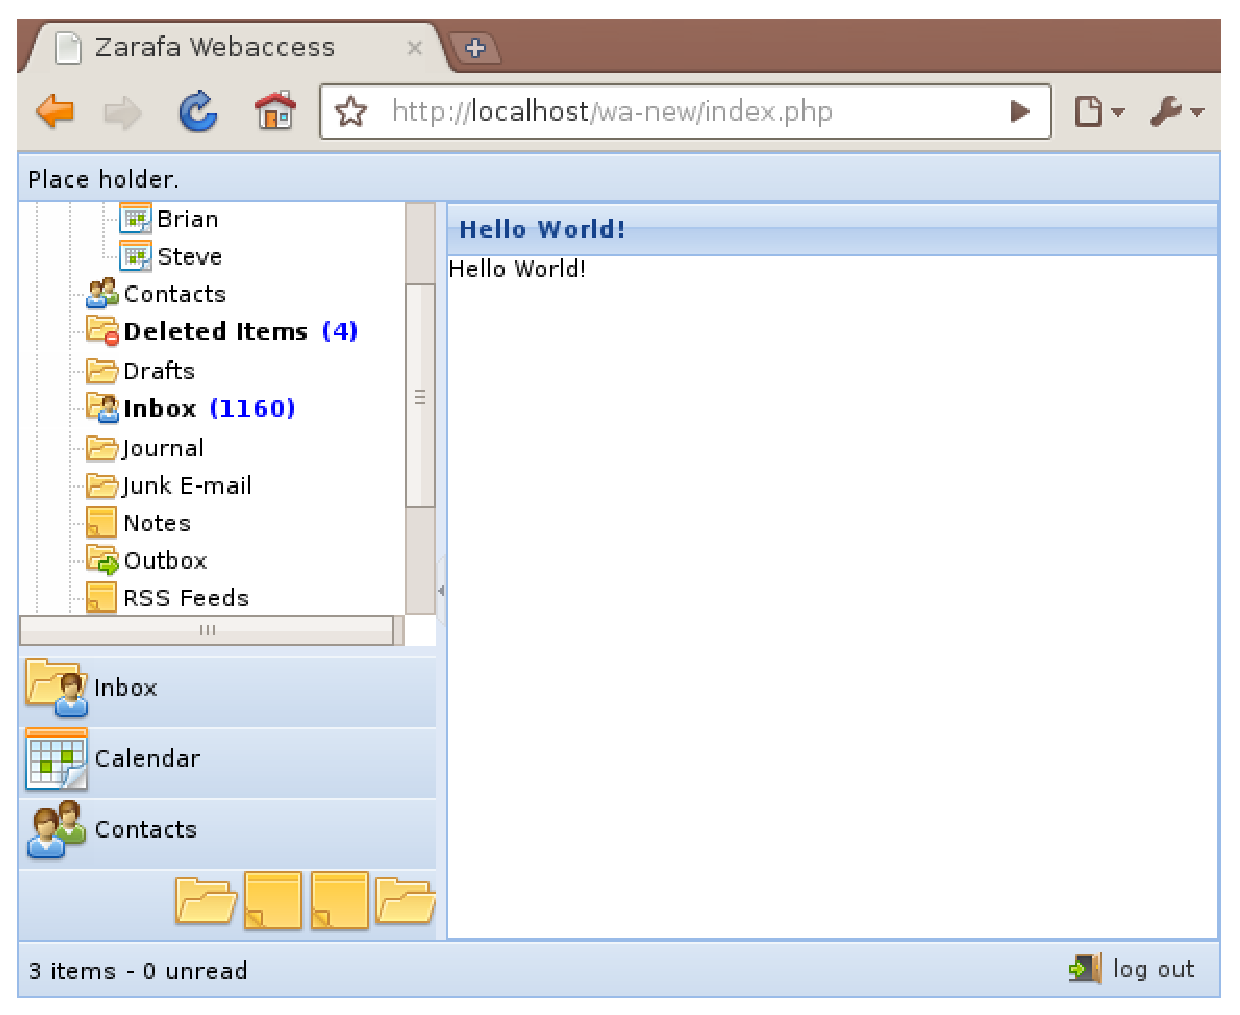
\includegraphics[width=9cm]{figures/taskcontext.eps}
\caption{Task context says hello.}
\label{figure:taskcontext}
\end{figure}

The next step is to retrieve tasks from the server and show them on screen. We do this by creating a grid panel
and attaching a store to it. Listing \ref{listing:taskcontext2} shows the modifed code. 

\begin{lstlisting}[caption={Adding a grid panel.}, label=listing:taskcontext2]
/**
 * @class Zarafa.ui.TaskContext
 * @extends Zarafa.ui.Context
 */
Zarafa.ui.TaskContext = function()
{
	var config = { name : 'taskcontext' };
	Zarafa.ui.TaskContext.superclass.constructor.call(this, config);
	
	// Convenience initialisation function.
	this.init();
};

Ext.extend(Zarafa.ui.TaskContext, Zarafa.ui.Context, {
	
	init : function()
	{
		// Create a store to hold our loaded task records.
		this.store = new Zarafa.comm.TaskStore();
	},
	
	// called when the context is enabled (the user clicks a task folder)
	enable : function(parameters)
	{
		this.store.load({
			storeId : parameters.store.id,
			entryId : parameters.folder.entryid
		});
	},
	
	// Create content panel.
	createContentPanel : function()
	{
		return new Ext.grid.GridPanel({
			border : false,
			
			viewConfig :
			{
				forceFit : true,
				showPreview : true,
				enableRowBody : true
			},

			// Column Model.
			cm : new Ext.grid.ColumnModel(
			[
				{
					dataIndex : 'owner',
					header : "Owner",
					sortable : true
				},
				{
					dataIndex : 'subject',
					header : "Subject",
					sortable : true
				}
			]),
            
			// Connect our store to the grid.
			store : this.store
		
		});
	},
	
	// bid() and createToolbar() omitted for brevity
	
});

container.registerPlugin(new Zarafa.ui.TaskContext());\end{lstlisting}

We first create an {\tt init} method that constructs a new instance of 
{\tt Zarafa.comm.TaskStore}. This is the store that will contain the task records displayed on the screen.
We want to load tasks into this store when a folder is selected by the user. To do this we
override the {\tt enable} method. It is automatically called by the framework when a context has
won the bidding round and just before its components are made visible. 
As with the {\tt bid} method, a parameter object is passed containing store and folder details.
We call {\tt load} on our store and pass it the MAPI ids of the store and folder so that it knows what to load.
Finally, to show the information to the user, we modify the {\tt createContentPanel} function to return a grid
panel, configured to show data from the store. 

\begin{figure}[h!]
\centering
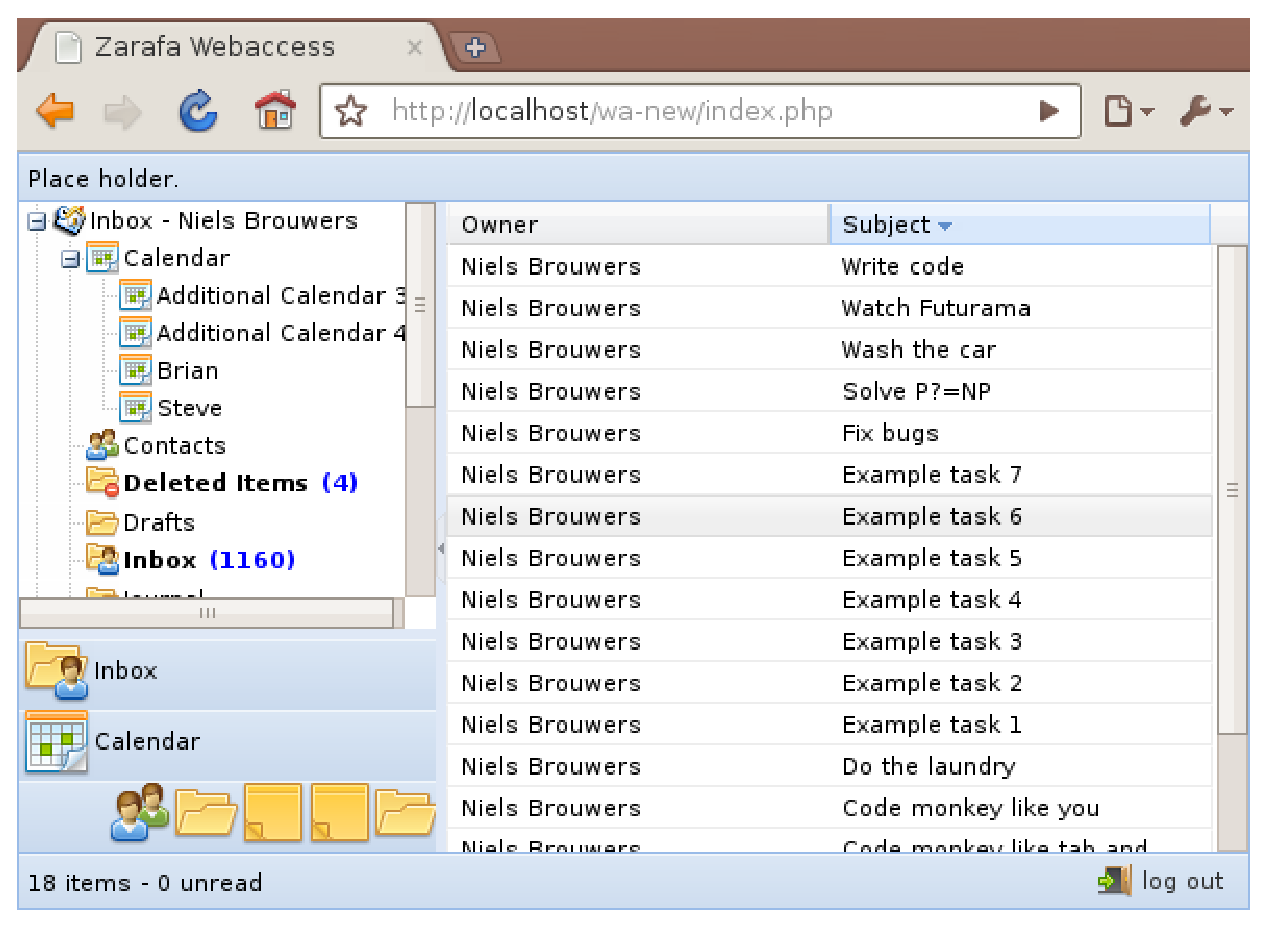
\includegraphics[width=9cm]{figures/taskcontext2.eps}
\caption{Task context with real data.}
\label{figure:taskcontext2}
\end{figure}

Figure \ref{figure:taskcontext2} shows the result. It is possible to sort by owner or subject by clicking the
corresponding column headers. The store will remember the store- and folder MAPI ids automatically, so that
subsequent load commands (in this case from the grid panel) collect the right data.

% \subsection{Adding a 'new' button}


